\documentclass{article} 
\usepackage{url, graphicx}
\usepackage[margin=1in]{geometry}
\usepackage{textcomp}
\usepackage{algpseudocode}
\usepackage{algorithm}
\usepackage{titling}
\usepackage{amsmath}
\usepackage{amssymb}
\usepackage{amsthm}
\usepackage{verbatim}
\usepackage{listings} % for code highlighting/formatting
\usepackage[final]{pdfpages}
\usepackage{color,soul}

\usepackage{color} %defining colors for syntax highlighting
\definecolor{syntaxBlue}{RGB}{42,0.0,255}
\definecolor{syntaxGreen}{RGB}{63,127,95}
\definecolor{syntaxPurple}{RGB}{127,0,85}
\definecolor{syntaxCyan}{RGB}{0,155,155}
\definecolor{syntaxGreyBg}{RGB}{220,220,220}


\lstset{
    basicstyle=\small\ttfamily, % Global Code Style
    tabsize=2, % number of spaces indented when discovering a tab 
    columns=fixed, % make all characters equal width
    keepspaces=true, % does not ignore spaces to fit width, convert tabs to spaces
    showstringspaces=false, % lets spaces in strings appear as real spaces
    breaklines=true, % wrap lines if they don't fit
    frame=trbl, % draw a frame at the top, right, left and bottom of the listing
    frameround=tttt, % make the frame round at all four corners
    framesep=4pt, % quarter circle size of the round corners
    numbers=left, % show line numbers at the left
    numberstyle=\tiny\ttfamily, % style of the line numbers
    commentstyle=\color{syntaxGreen},
    keywordstyle=\color{syntaxPurple},
    stringstyle=\color{syntaxBlue},
    emph={int,char,float,struct,string},
    emphstyle=\color{syntaxCyan},
    backgroundcolor=\color{syntaxGreyBg},
}

\title{Psychic Waffle Project Proposal}
\author{
    A.J. Feather\\
    \texttt{af2849@columbia.edu}
    \and
    Andrew Grant\\
    \texttt{amg2215@columbia.edu}
    \and
    Jacob Graff\\
    \texttt{jag2302@columbia.edu}
    \and
    Jake Weissman\\
    \texttt{jdw2159@columbia.edu}
}
\date{\today}

\begin{document}

\maketitle

\section{Synopsis}

\subsection{Motivation}
Large buy/sell orders have the potential to significantly move markets if not executed properly. Big orders that are executed in a single trade can adversely push the market price against the trader. For example, if a trader shows he or she has a large sell order, the relevant asset's price will almost inevitably move lower; this will result in the trader selling at an average lower price. The goal of this project is to build a system that accounts for these market dynamics and executes client orders as optimally as possible for them. By filling orders on their behalf \emph{and} at the optimal price, our clients will save time and money. 

\subsection{Functionality} % What will it do?
Our system will receive a customer order, figure out the most optimal method of execution (it will usually split the order up into increments), and fill the order. The heart of the system will be an algorithm that figures out the most optimal method of execution: given X shares left to sell at time Y, the system will determine the next sell order. This requires the system to calculate when to execute the next sale of shares, as well as how many shares to sell at the current price. Furthermore, the system will provide the user with immediate feedback detailing each execution attempt. More specifically, after each execution attempt, the system will respond with whether the order was filled or not, and if the order was filled how many shares were traded and at what average price. \hl{We also plan to provide the ability for the trader who placed the transaction to monitor the progress of the transaction as it is being executed throughout the day.}

\subsection{Users}
Since the system was requested by a Pension Fund, this will be our primary user for now. Furthermore, our system is designed to handle large sell orders for customers who are happy to get their orders done over the course of the day (as opposed to instantaneously). Nonetheless, anyone trading Acme on this exchange, who needs similar types of orders filled should be able to use our system. This would include Hedge Funds, Banks, Individual Traders, Brokers and other financial professionals/firms. \hl{While the platform will accommodate those entities, the specific user interfacing with our platform will be a trader who will be executing the transaction on behalf of their client.  The system will initially support a single user to place and monitor trades and will eventually scale up to accommodate more traders to use the system concurrently.}

\subsection{Usage}
As of now the client's main use of our system will be to execute large sell orders. \hl{The additional features we plan to provide are better monitoring tools and potentially an improved visualization platform as a stretch goal.}

\pagebreak
\subsection{User Stories}

\subsubsection{User Login}

The user should be able to log in to the platform with unique user credentials.

\subsubsection{Request Number of Shares}

Users will need to be able to retrieve the number of total shares available for sale.

\subsubsection{Request Best/Worst Sell Price Available}

In case the user wants to buy at a particular point in time, we will give them the ability to request the best and worst available buy prices. 

\subsubsection{Submit Sell Order}

The user should be able to send a sell order to the system, giving a sale price and the number of shares thaneed to be soldld.

\subsection{Sell Order Work Flow}

The largest back end challenge we face at this time is attempting to match the user's specified price. To handle this, we plan on using a form of the VWAP algorithm. The following diagram shows that workflow (on the next page).

\begin{figure}
   \centering
   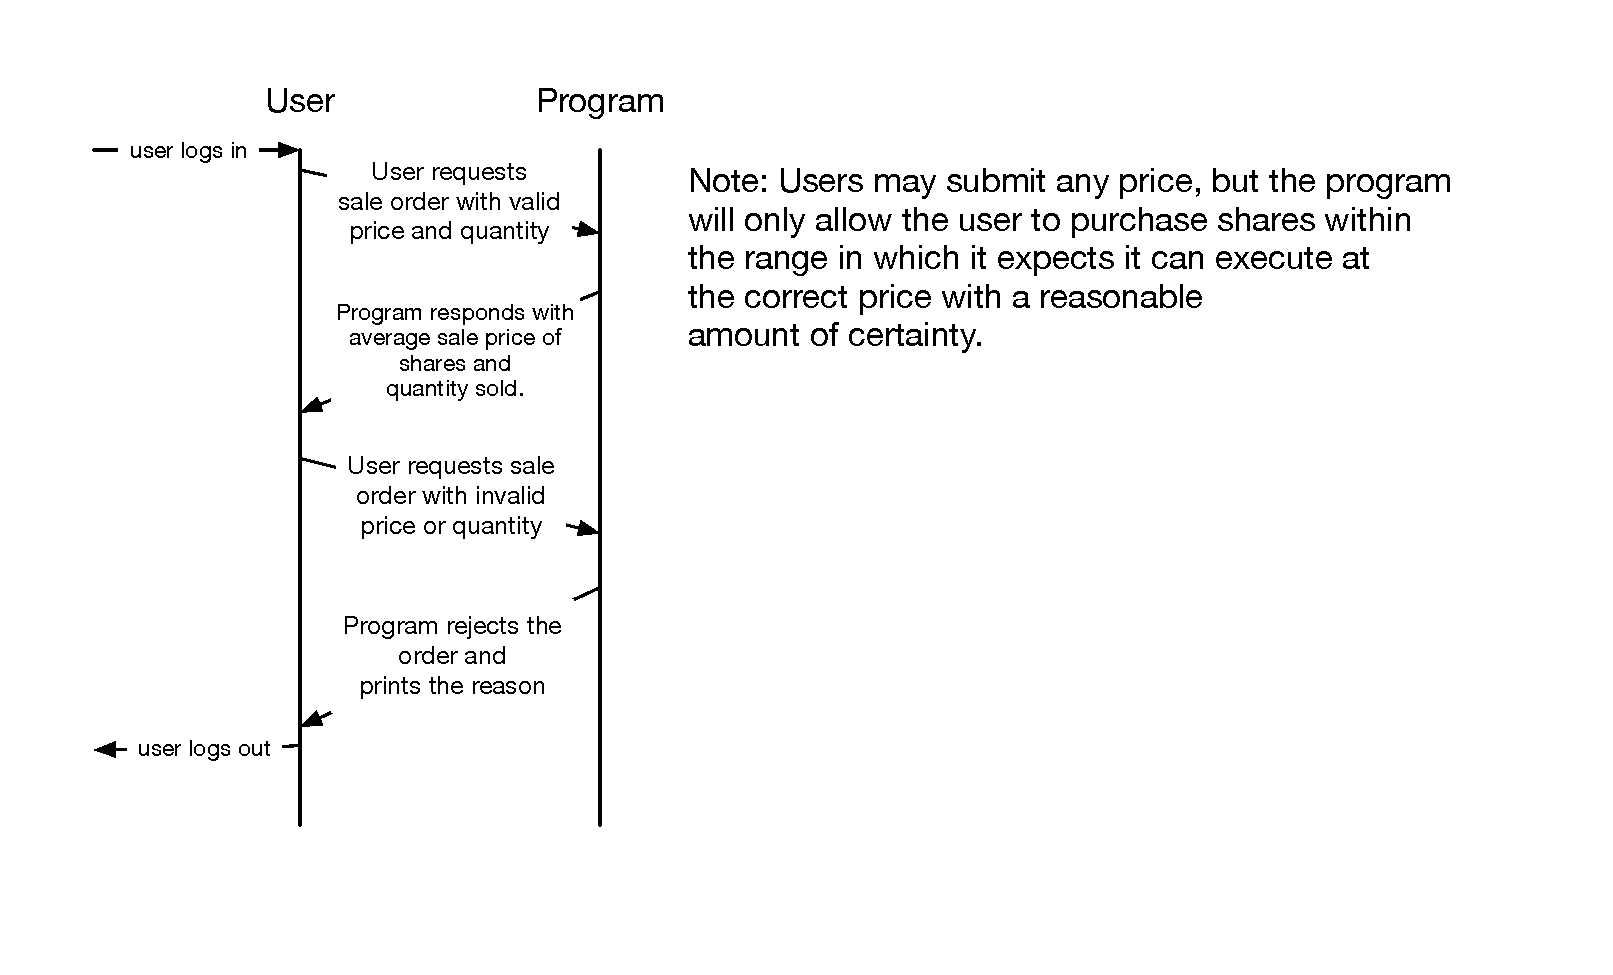
\includepdf[pages=-, offset=0 -150]{proposal_diagram.pdf}
\end{figure}

\pagebreak
\subsection{Error Handling}

\paragraph{}

We will do our best to provide the user with the ability to report unexpected behavior at any point. We will also write tests that cover most essential features that will log errors while the program is running in addition to the full testing suite.\\

These logs will include issues such as failed connections and unexpected return values.\\

We also plan to cleanse all text as it is entered into the program.

\section{Technology}

\subsection{Programming Language}
The bulk of our code will be written in python - python has many easily accessible dev tools, and can for many applications substantially decrease development time. 
\subsection{Development Framework}
Our development framework will be flask (http://flask.pocoo.org/), a web development framework, which allows webservers to be created quite easily, and gives a lot of flexibility to the developers. \\
\\
In addition, we will use pip, the python package manager, to install the packages we need, and virtualenv in order to properly maintain our python environment. 
\subsection{Build Automation Tool}
Our preliminary build automation tool will be PyBuilder (https://pybuilder.github.io/).
\subsection{Static Analysis Tool}
Our preliminary static analysis tool will be Pylint (https://www.pylint.org/), a popular linter for python.
\subsection{Unit testing tool}
Our preliminary unit testing tool will be PyUnit, the unit testing tool that is built in to python.
\subsection{Persistent Data Store} 
Our persistant data store will be a PostgresQL database, in which we will store (at least initially) user data and password hashes.
\end{document} 